% THIS IS AN EXAMPLE DOCUMENT FOR VLDB 2012
% based on ACM SIGPROC-SP.TEX VERSION 2.7
% Modified by  Gerald Weber <gerald@cs.auckland.ac.nz>
% Removed the requirement to include *bbl file in here. (AhmetSacan, Sep2012)
% Fixed the equation on page 3 to prevent line overflow. (AhmetSacan, Sep2012)

\documentclass{vldb}
\usepackage{graphicx}
\usepackage{balance}  % for  \balance command ON LAST PAGE  (only there!)
\usepackage{times,amsmath,epsfig}
\usepackage{color}
\newtheorem{Definition}{Definition}{\itshape}{\rmfamily}
\newtheorem{Theorem}{Theorem}{\itshape}{\rmfamily}
\newcommand{\todo}[1]{{\footnotesize \textcolor{red}{$\ll$\textsf{TODO #1}$\gg$}}}
\newcommand{\bluefont}[1]{\textcolor{blue}{#1}}
\newcommand{\redfont}[1]{\textcolor{red}{#1}}
\newcommand{\greenfont}[1]{\textcolor{green}{#1}}
\newcommand{\yellowfont}[1]{\textcolor{yellow}{#1}}


% Include information below and uncomment for camera ready
\vldbTitle{Pixels: Adaptive Column Store for Wide Table Analysis}
\vldbAuthors{Haoqiong Bian, Guodong Jin, Yueguo Chen, Xiaoyong Du, Xiongpai Qin}
\vldbDOI{https://doi.org/TBD}

\begin{document}
	
	% ****************** TITLE ****************************************
	
	\title{Pixels: Adaptive Column Store for Wide Table Analysis}
	
	
	% possible, but not really needed or used for PVLDB:
	%\subtitle{[Extended Abstract]
	%\titlenote{A full version of this paper is available as\textit{Author's Guide to Preparing ACM SIG Proceedings Using \LaTeX$2_\epsilon$\ and BibTeX} at \texttt{www.acm.org/eaddress.htm}}}
	
	% ****************** AUTHORS **************************************
	
	% You need the command \numberofauthors to handle the 'placement
	% and alignment' of the authors beneath the title.
	%
	% For aesthetic reasons, we recommend 'three authors at a time'
	% i.e. three 'name/affiliation blocks' be placed beneath the title.
	%
	% NOTE: You are NOT restricted in how many 'rows' of
	% "name/affiliations" may appear. We just ask that you restrict
	% the number of 'columns' to three.
	%
	% Because of the available 'opening page real-estate'
	% we ask you to refrain from putting more than six authors
	% (two rows with three columns) beneath the article title.
	% More than six makes the first-page appear very cluttered indeed.
	%
	% Use the \alignauthor commands to handle the names
	% and affiliations for an 'aesthetic maximum' of six authors.
	% Add names, affiliations, addresses for
	% the seventh etc. author(s) as the argument for the
	% \additionalauthors command.
	% These 'additional authors' will be output/set for you
	% without further effort on your part as the last section in
	% the body of your article BEFORE References or any Appendices.
	
	\numberofauthors{5} %  in this sample file, there are a *total*
	% of EIGHT authors. SIX appear on the 'first-page' (for formatting
	% reasons) and the remaining two appear in the \additionalauthors section.
	
	\author{
		% You can go ahead and credit any number of authors here,
		% e.g. one 'row of three' or two rows (consisting of one row of three
		% and a second row of one, two or three).
		%
		% The command \alignauthor (no curly braces needed) should
		% precede each author name, affiliation/snail-mail address and
		% e-mail address. Additionally, tag each line of
		% affiliation/address with \affaddr, and tag the
		% e-mail address with \email.
		%
		% 1st. author
		\alignauthor
		Haoqiong Bian\\%\titlenote{Dr.~Trovato insisted his name be first.}\\
		\affaddr{School of Information,\\Renmin University of China}\\
		%\affaddr{1932 Wallamaloo Lane}\\
		%\affaddr{Wallamaloo, New Zealand}\\
		\affaddr{Beijing, China}\\
		\email{bianhq@ruc.edu.cn}
		% 2nd. author
		\alignauthor
		Guodong Jin\titlenote{Guodong Jin and Haoqiong Bian contributed equally to this work.}\\
		\affaddr{School of Information,\\Renmin University of China}\\
		%\affaddr{P.O. Box 1212}\\
		%\affaddr{Dublin, Ohio 43017-6221}\\
		\affaddr{Beijing, China}\\
		\email{jinguodong@ruc.edu.cn}
		% 3rd. author
		\alignauthor Yueguo Chen
		\titlenote{Yueguo Chen is the corresponding author.}\\
		\affaddr{School of Information,\\Renmin University of China}\\
		%\affaddr{1 Th{\large{\sf{\o}}}rv{$\ddot{\mbox{a}}$}ld Circle}\\
		%\affaddr{Hekla, Iceland}\\
		\affaddr{Beijing, China}\\
		\email{chenyueguo@ruc.edu.cn}
		%\and  % use '\and' if you need 'another row' of author names
	}
	% There's nothing stopping you putting the seventh, eighth, etc.
	% author on the opening page (as the 'third row') but we ask,
	% for aesthetic reasons that you place these 'additional authors'
	% in the \additional authors block, viz.
	\additionalauthors{
		Additional authors: \\
		Xiaoyong Du
		(School of Information, Renmin University of China, {\texttt{duyong@ruc.edu.cn}}), \\
		Xiongpai Qin
		(School of Information, Renmin University of China, { \texttt{qxp1990@ruc.edu.cn}})}
	\date{30 July 1999}
	% Just remember to make sure that the TOTAL number of authors
	% is the number that will appear on the first page PLUS the
	% number that will appear in the \additionalauthors section.
	
	
	\maketitle
	
	\begin{abstract}
		The abstract for your paper for the PVLDB Journal submission.
		The template and the example document are based on the ACM SIG Proceedings  templates. This file is part of a package for preparing the submissions for review. These files are in the camera-ready format, but they do not contain the full copyright note.
		Note that after the notification of acceptance, there will be an updated style file for the camera-ready submission containing the copyright note.
	\end{abstract}


\section{Introduction}

\todo{Write later. 1) What is wide table and where it is used; 2) Why do we use wide tables instead of normal tables; 3) What are the problems we try to solve in this paper; 4) Challenges; 5) Our achievements and contributions}

\subsection{Background}

\subsection{Goals}

\subsection{Contributions}

\section{Preliminaries}

In this section, we review today's HDFS-based column stores in which wide tables are stored, and how queries are executed on top of these wide tables \cite{IEEEexample:IEEEwebsite}.

\subsection{Disk Seek Cost}

\subsection{Wide Table Layout in HDFS}
\todo{1) columnar format in HDFS; 2) wide tables are store in these formats; 3) disk seek cost problem.}


\subsection{Query Execution on Wide Tables}

\todo{1) one task per split / row group; 2) task schedule and initialization cost; 3) adaptive split size problem.}



\section{Challenges}
We address the challenges of wide table analysis.
\subsection{Workload Modeling}

\subsection{Column Chunk Ordering}
Effective column chunk ordering strategies shall satisfy following constraints:
\begin{enumerate}
	\item Colocate frequently paired visited column chunks as close as possible physically.
	\item Tradeoff between ordering and reconstruction.
\end{enumerate}
\subsection{Data Splitting}

\subsection{Column Chunk Caching}
Nowadays commonly used cache mechanism on HDFS is based on its block, caching on more precise units such as column chunks can help improve query performance.

\section{System Overview}

Pixels is an adaptive storage system on top of HDFS.
As shown in Figure~\ref{fig:overview}, it contains six functional modules:
\begin{itemize}
	\item \textit{Data Ingestion}. Unlike traditional ETL process on HDFS in which data is transformed into specific format in a batch manner, in Pixels, data is ingested into the system in a streaming manner.
	We assume that the analytical workload mostly accesses the most recent data, so that we do not reload the historical data.
	When the Layout generator generates a new data layout, it is only applied on the new coming data.
	
	\item \textit{Workload Modeling}. Workload modeling is responsible for collecting the query workload and build workload models. Access patterns (columns accessed by queries) and filters (predicates) of the queries are collected by this module.
	Then the access patterns and filters are used to build a workload model by which we can predict the access patterns and filters in the coming future. In pixels, we use hidden Markov chain to model the workload.
	
	\item \textit{Layout Generator}. Layout generator optimizes the data layout with the workload model built by \textit{Workload Modeling} module and the reading cost model built by \textit{Reading Cost Modeling}.
	Data layout optimization is triggered by workload modeling module when the workload model is significantly changed.
	The new data layout generated and evaluated by layout generator is then provided to \textit{Data Ingestion} module to be applied in the new coming data.
	
	\item \textit{Data Split Generator}. Each data reading task reads a data split.
	Traditionally, each mapper task reads a HDFS block as a data split by default, while in Pixels, the data split is adaptively generated by data split generator, which takes both of task execution parallelism and HDFS block size into consideration.

	\item \textit{Column Chunk Caching}. Column chunk caching is a local cache manager for column chunks in Pixels files. 
	Compared with HDFS block as the default cache unit, column chunk is a much smaller storage unit, and can improve cache hitting rate greatly.
	
	\item \textit{Reading Cost Modeling}. Reading cost modeling moudle collects and maintains disk reading costs, which are used to build the data reading cost model.
	The model is sent to \textit{Layout Generator} for layout optimization.
	Data statistics are also collected and maintained and used by \textit{Data Split Generator} to optimize data splits of reading tasks and used by \textit{Data Ingestion} module to optimize data encoding and indexing.
\end{itemize}

\begin{figure}[h!]
	\vspace{-1em}
	\centering
	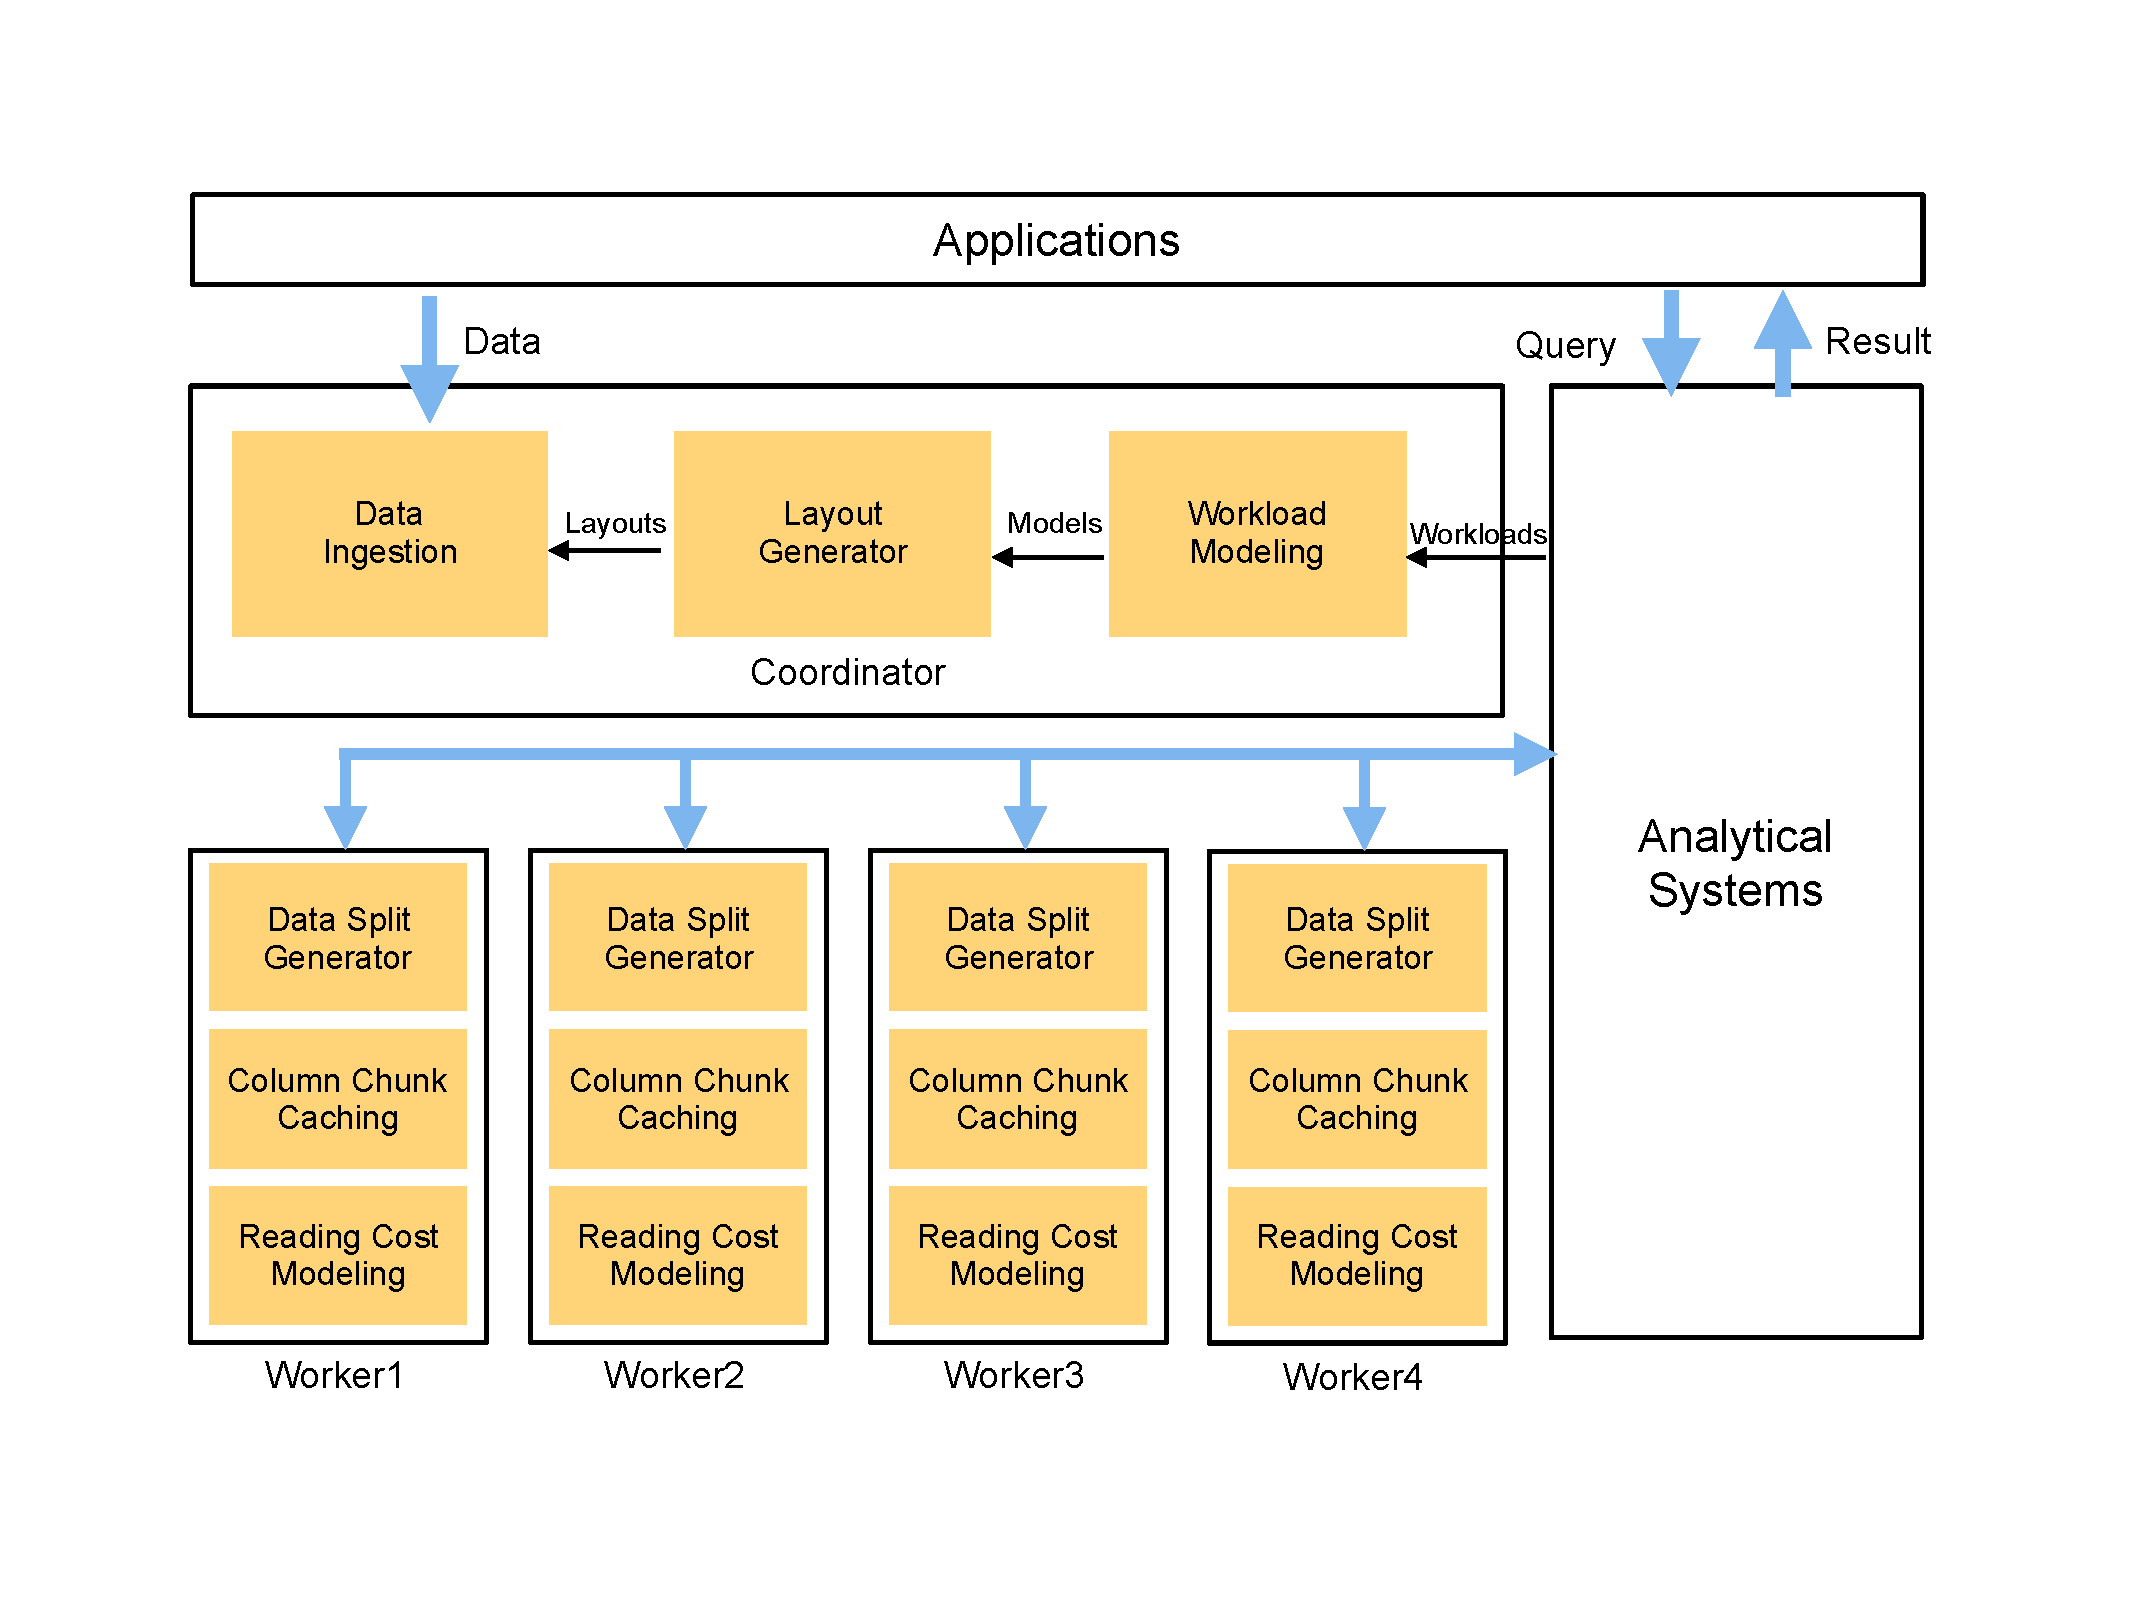
\includegraphics[width=0.5\textwidth, height=0.36\textwidth]{figs/framework}
	\vspace{-3em}
	\caption{System Framework of Pixels}\label{fig:overview}
	\vspace{-0em}
\end{figure}

As a whole system, \textit{Workload Modeling}, \textit{Layout Generator} and \textit{Data Ingestion} modules are located on \textit{Coordinator} node in the cluster. \textit{Data Split Generator}, \textit{Column Chunk Caching} and \textit{Reading Cost Modeling} modules are resided on each worker node.

User data are ingested by data ingestion module in a streaming manner.
Meanwhile, queries are submitted to analytical systems, e.g. Spark SQL, Presto, and query workloads are collected by workload modeling module.
Upon significant change of workload model, layout generator module optimizes data layout based on new workload model and then generates a new data layout, which is applied in data ingestion module in the new coming data.
During query execution, analytical systems get the data split strategy through data split generator module, and then data reading tasks access column chunks through column chunk caching module.
When cache missing happens, column chunk caching module is responsible for reading column chunks from disk into caching buffer. During cache accessing and disk reading, reading cost modeling module collects and maintains data statistics and disk reading costs.


\section{Layout Optimization}
\label{sec:layout-optimization}

\subsection{Workload Modeling}
\label{subsec:workload-modeling}
Assumptions:
\begin{itemize}
	\item Mostly queries access most recent ingested data.
	\item Patterns of query access paths evolves slowly instead of abruptly.
\end{itemize}

Goals:
\begin{itemize}
	\item Detect changes of access paths, and decide to propose a new round of optimization.
	\item Analyze patterns of access paths.
\end{itemize}

Basic idea: Reading optimizer collects access column chunks of each query, and send to layout optimizer.

\subsection{Column Chunk Ordering}
\label{subsec:column-chunk-ordering}
Local cache buffer.

\section{Reading Optimization}
\label{sec:reading-optimization}


\subsection{Data Split Generator}
\label{subsec:data-splitting}
The goal of data split generator is to adaptively assign row groups to data splits when query comes.
When assigning row groups, the generator takes local task parallelism, memory size and query access patterns into consideration. 

\subsection{Column Chunk Caching}
\label{subsec:chunk-caching}


\section{Implementation}
\label{sec:impl}
\subsection{Pixels File Format}
Pixels is the underlying file format supporting optimized storage of wide tables in system.
The file format is similar to ORC and Parquet logically.

\subsection{Row Group Compactor}


\section{Performance Evaluation}
\label{sec:exp}

\section{Related Work}
\label{sec:related}

\section{Conclusion}



% The following two commands are all you need in the
% initial runs of your .tex file to
% produce the bibliography for the citations in your paper.
\bibliographystyle{abbrv}
\bibliography{acm-ref}  % vldb_sample.bib is the name of the Bibliography in this case
% You must have a proper ".bib" file
%  and remember to run:
% latex bibtex latex latex
% to resolve all references

%\subsection{References}
%Generated by bibtex from your ~.bib file.  Run latex,
%then bibtex, then latex twice (to resolve references).

%APPENDIX is optional.
% ****************** APPENDIX **************************************
% Example of an appendix; typically would start on a new page
%pagebreak

\begin{appendix}
	You can use an appendix for optional proofs or details of your evaluation which are not absolutely necessary to the core understanding of your paper. 
	
	\section{Final Thoughts on Good Layout}
	Please use readable font sizes in the figures and graphs. Avoid tempering with the correct border values, and the spacing (and format) of both text and captions of the PVLDB format (e.g. captions are bold).
	
	At the end, please check for an overall pleasant layout, e.g. by ensuring a readable and logical positioning of any floating figures and tables. Please also check for any line overflows, which are only allowed in extraordinary circumstances (such as wide formulas or URLs where a line wrap would be counterintuitive).
	
	Use the \texttt{balance} package together with a \texttt{\char'134 balance} command at the end of your document to ensure that the last page has balanced (i.e. same length) columns.
	
\end{appendix}

\balance

\end{document}
